\cleardoublepage

\chapter{Dream recall frequency}
\label{sec:dream-recall}

\cleanchapterquote{We must also inquire what the dream is, and from what cause sleepers sometimes dream, and sometimes do not; or whether the truth is that sleepers always dream but do not always remember (their dream); and if this occurs, what its explanation is.}{Aristotle}{On dreams. 350 B.C.}

\section{Measuring dream recall frequency}
\label{sec:dream-recall:method}

As Aristotle had rightly pointed out, we do not always remember our dreams. More than two thousand years after, modern research has confirmed that the dream recall frequency (DRF) – i.e. the number of dream reports over a given period of time -  is indeed highly variable both within individuals over the life course, but also between individuals \citep{schredl_factors_2003, ruby_experimental_2011}.
There is no gold standard for measuring DRF, and each method has its pros and cons. In research settings, three methods are commonly applied: questionnaire scales, dream diaries, and laboratory awakenings \citep{schredl_dream_1999}. The former consists in simply asking the participants to estimate their dream recall frequency over the last few weeks or months. This method has the advantage of being fast, inexpensive, and unaffected by the measurement, however, the DRF could be over- or under-estimated due to erroneous or incomplete recollection. Regarding dream diaries, the participants are asked to report each morning whether they have recalled a dream or not. This method minimizes the bias of retrospective estimation, but has the disadvantages of potentially increasing drastically the dream recall frequency, especially in persons who usually almost never recall their dreams \citep{schredl_questionnaires_2002}. Finally, laboratory awakenings consist in awakening the participants in the sleep lab and asking them whether they recall a dream or not. While this method has the clear advantage that the experimenters can measure physiological parameters (EEG, EOG, ECG, respiration and heart rate) prior, during and after the awakening, it is also time-consuming and expensive. Moreover, as for dream diaries, laboratory awakenings are associated with a dramatic increase in DRF, especially for low dream recallers.

\section{DRF in the general population}
\label{sec:dream-recall:pop}

\subsection{Average DRF}
\label{sec:dream-recall:pop:avg}

Measured by questionnaire, the average weekly DRF was 2.58 ± 2.03 in 444 German students \citep{schredl_factors_2003} and 0.83 ± 1.57 in a representative German sample of 931 participants \citep{schredl_dream_2008}. Using dream diaries, the average weekly DRF was 3.1 ± 1.5 in 70 Finnish children \citep{valli_threat_2005} and 3.9 ± 2.5 in a sample of 196 German student \citep{schredl_reliability_2005}. In lights of these results, we can conclude that the average weekly DRF in the general population lies between 1 and 3 dream reports per week.

\subsection{Intra-individuals variability}
\label{sec:dream-recall:pop:intra}

Daily experience suggest that our ability to recall dream fluctuate over time. Investigating this issue using the diary technique in 169 participants, \citet{schredl_reliability_2005} reported that the stability of DRF was very high over a period of one month. Similarly, he reported high DRF stability coefficients in a sample of older adults who had been interviewed weekly about their dream life over a period of 26 weeks \citep{schredl_reliability_2001}. However, to our knowledge, there are no studies evaluating the stability of DRF in the same individuals over an extended period of time.

\subsection{Inter-individuals variability}
\label{sec:dream-recall:pop:inter}

DRF vary drastically between individuals: some persons almost never recall a dream, whereas others can relate one or several dreams every morning. In an Austrian sample of 1000 persons, \citet{stepansky_austrian_1998} found that 31\% of the participants reported 10 dreams or more per month, 37\% reported between one and nine dreams per month, and 32\% reported less than one dream per month. In a sample of 285 German students, \citet{schredl_questionnaires_2002} found that 44\% reported dreams four or more times per weeks, 44\% reported a dream one time per week and 12\% reported a dream less than one time per month. This variability allows to differentiate behavioral profiles of DRF: high dream recallers (HR), who can relate a dream almost every morning (e.g. more than 5 times a week, \citealp{schredl_reliability_2005}) and low dream recallers (LR), who almost never recall a dream (e.g. less than one dream per month, \citealp{goodenough_comparison_1959}). Importantly, the frequency of HR is higher in the general population, and even more in young and/or student sample \citep{schredl_reliability_2005}.

\section{Parameters correlated with DRF}
\label{sec:dream-recall:param}

\subsection{Psychological factors}
\label{sec:dream-recall:param:psych}

First, increased professional or personal stress is positively associated with DRF \citep{schredl_dream_1999}. Similarly, an interest in dreams, or a positive attitude towards dreams in general is clearly associated with DRF, as is frequent day-dreaming and rich fantasy life \citep{schredl_factors_2003}. DRF decreases with age and tends to be higher in women, who are also typically more interested in dreams \citep{schredl_dream_2008, schredl_gender_2008}. Regarding personality dimensions, studies have found positive correlations between DRF and thin boundaries, anxiety, and openness to experience. However, most of the correlations between DRF and personality traits are low and explain only a small percentage of the total variance. Regarding cognitive abilities, several studies have consistently reported that DRF is positively correlated with creativity. A simple explanation of why individuals differ in their ability to remember dreams could be because they differ in some more general memory abilities (verbal, visual, short and long term). However, the literature yielded contradictory results, with some support for a positive association between DRF and visual memory, but also evidence against it for verbal and visual material and short-or long-term story narrative recall \citep{ruby_experimental_2011, blagrove_trait_2010}.

\subsection{Sleep parameters}
\label{sec:dream-recall:param:sleep}

First, DRF varies according to the sleep stage preceding awakening (see \citealp{nielsen_review_2000} for a review). More dream reports are obtained after an awakening during REM sleep than after an awakening during NREM sleep. These results inspired the REM sleep hypothesis of dreaming discussed earlier in this thesis. However, when a dream is not reported on awakening, there is no method of establishing whether it did not happen or was forgotten. This idea was rightly pointed out by \citet{conduit_poor_2004}: \q{An ongoing assumption made by sleep scientists is that since dreams are more often recalled on awakening from REM sleep, dreams must occur more often during this sleep stage. An alternative hypothesis is that cognition occurs throughout sleep, but the recall of mentation differs on awakenings}.
This idea that DRF variability is not a matter of dream production during sleep, but of dream recall during awakening, is the core of several models of dream recall (detailed later in section \ref{sec:dream-recall:theories}), among which the arousal-retrieval model is one of the most significant. In its simplest form, it claims that a period of wakefulness must occur just after dreaming so that the dream content can be transferred from short term to long term memory \citep{koulack_dream_1976}
Several studies support this model. First, using retrospective evaluation, \citet{schredl_factors_2003} found a positive correlation between the number of nocturnal awakenings and DRF. Second, \citet{de_gennaro_recovery_2010} reported that recovery sleep following a full night of sleep deprivation was characterized by an almost complete abolition of dream recall, paralleled with a lower number of nocturnal awakenings, which could, according to them, have \q{reduced the contents available in memory as possible cues for retrieval of dream experiences at morning}. Finally, these results were recently reinforced by a full-night PSG study in 36 subjects (18 HR and 18 LR; \citealp{eichenlaub_brain_2014}; Figure \ref{fig:intro:jbe-sleep}). HR showed in average longer intra-sleep wakefulness than LR (~15min more on average). The number of awakenings (the number of phases composed of consecutive pages of awakening) was not significantly different between the 2 groups, but the mean duration of the awakenings was (HR, 1.90 ± 0.91 min; LR, 0.95 ± 0.40 min).

\begin{figure}[htb]
	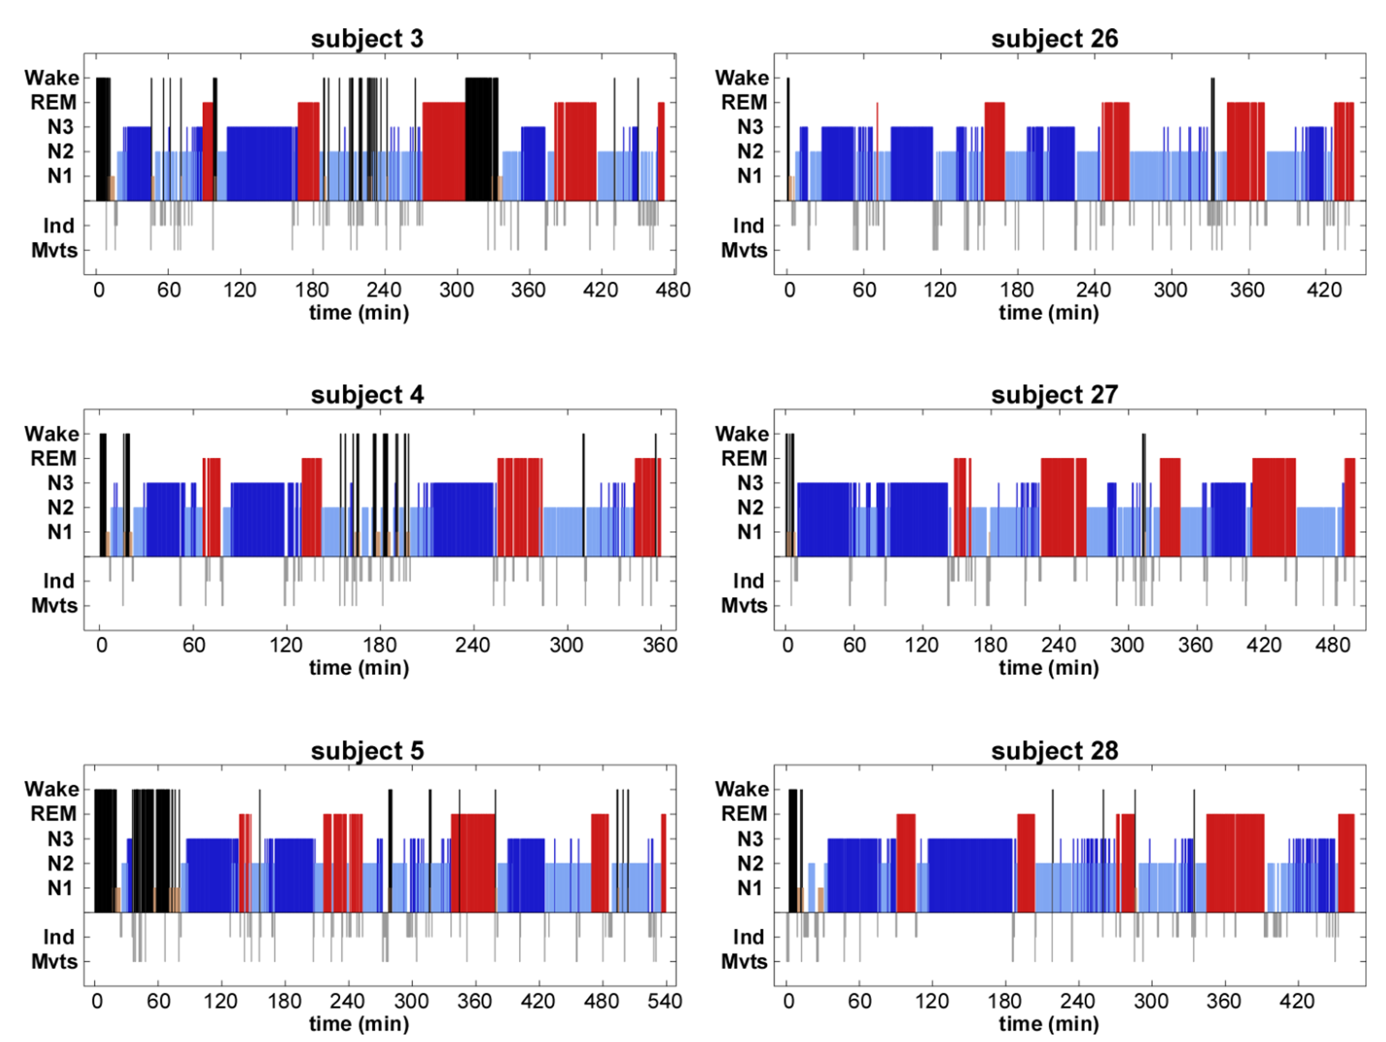
\includegraphics[width=\textwidth]{Fig/Intro/Intro_JBE_sleep/Intro_JBE_sleep.png}
	\caption[Hypnograms of typical high and low dream recallers]{Hypnograms of three representative HR (left) and three representative LR (right). Full night PSG recordings were acquired in the sleep lab in 18 HRs and 18 LRs. Wake: wakefulness (black); N1, N2, and N3: sleep stages N1 (very light gray), N2 (light gray), and N3 (dark gray), respectively; REM: REM sleep (medium gray); Ind: pages for which the dominant sleep stage could not be determined; Mvts: movements. From these 6 examples, it can be observed that the wakefulness periods during the sleep period time are longer in HR than in LR. Adapted from \citet{eichenlaub_brain_2014}}
	\label{fig:intro:jbe-sleep}
\end{figure}

\subsection{Neurophysiological parameters}
\label{sec:dream-recall:param:neuro}

The neurophysiological parameters that covary with DRF had never been investigated until the doctoral work of Jean-Baptiste Eichenlaub, conducted with Perrine Ruby a few years ago. The present study follows on from this work, in which they compared the brain activity of HR and LR during both sleep and wakefulness and using several neuroimaging techniques such as auditory evoked potentials (AEP) and positron emission tomography (PET). The main findings from his Eichenlaub’s doctoral thesis are summarized in Figure \ref{fig:intro:jbe-summary}.
First, they conducted a sleep lab study in which they compared the brain reactivity (AEP) of 18 HRs (DRF = 4.4 ± 1.0 dream reports per week) and 18 LRs (0.25 ± 0.1) during sleep and wakefulness \citep{eichenlaub_brain_2014}. During data acquisition, the subjects were presented with sounds to be ignored (first names randomly presented among pure tones) while they were watching a silent movie or sleeping. They found that brain responses to first names dramatically differed between the 2 groups during both sleep and wakefulness (Figure \ref{fig:intro:jbe-summary}A). During wakefulness, the attention-orienting brain response (P3a) and a late parietal response were larger in HR than in LR. During sleep, there were between-group differences at the latency of the P3a during N2 sleep and at later latencies during all sleep stages.
Second, they used PET to compare the resting state cerebral blood flow of 21 HRs (DRF = 5.2 ± 1.4 dream reports per week) and 20 LRs (DRF = 0.5 ± 0.3 dream reports per week) during sleep and wakefulness \citep{eichenlaub_resting_2014}. Compared with LRs, HRs showed higher rCBF in the TPJ during REM sleep, N3, and wakefulness, and in the MPFC during REM sleep and wakefulness (Figure \ref{fig:intro:jbe-summary}B).
Altogether, these findings show that HR and LR have different neurophysiological traits: spontaneous and evoked brain activity of HR and LR differ during wakefulness and sleep. They argued that HR’s neurophysiological profile could promote mental imagery during sleep and the encoding or retrieval of the dream memory during wakefulness. Notably, increased attention-orienting responses during sleep in HR could increase the proportion of intra-sleep awakenings, which in turn would facilitate the encoding of dreams according to the arousal-retrieval model, and finally result in a higher likelihood of dream recall in the morning after awakening.

\begin{figure}[!htb]
	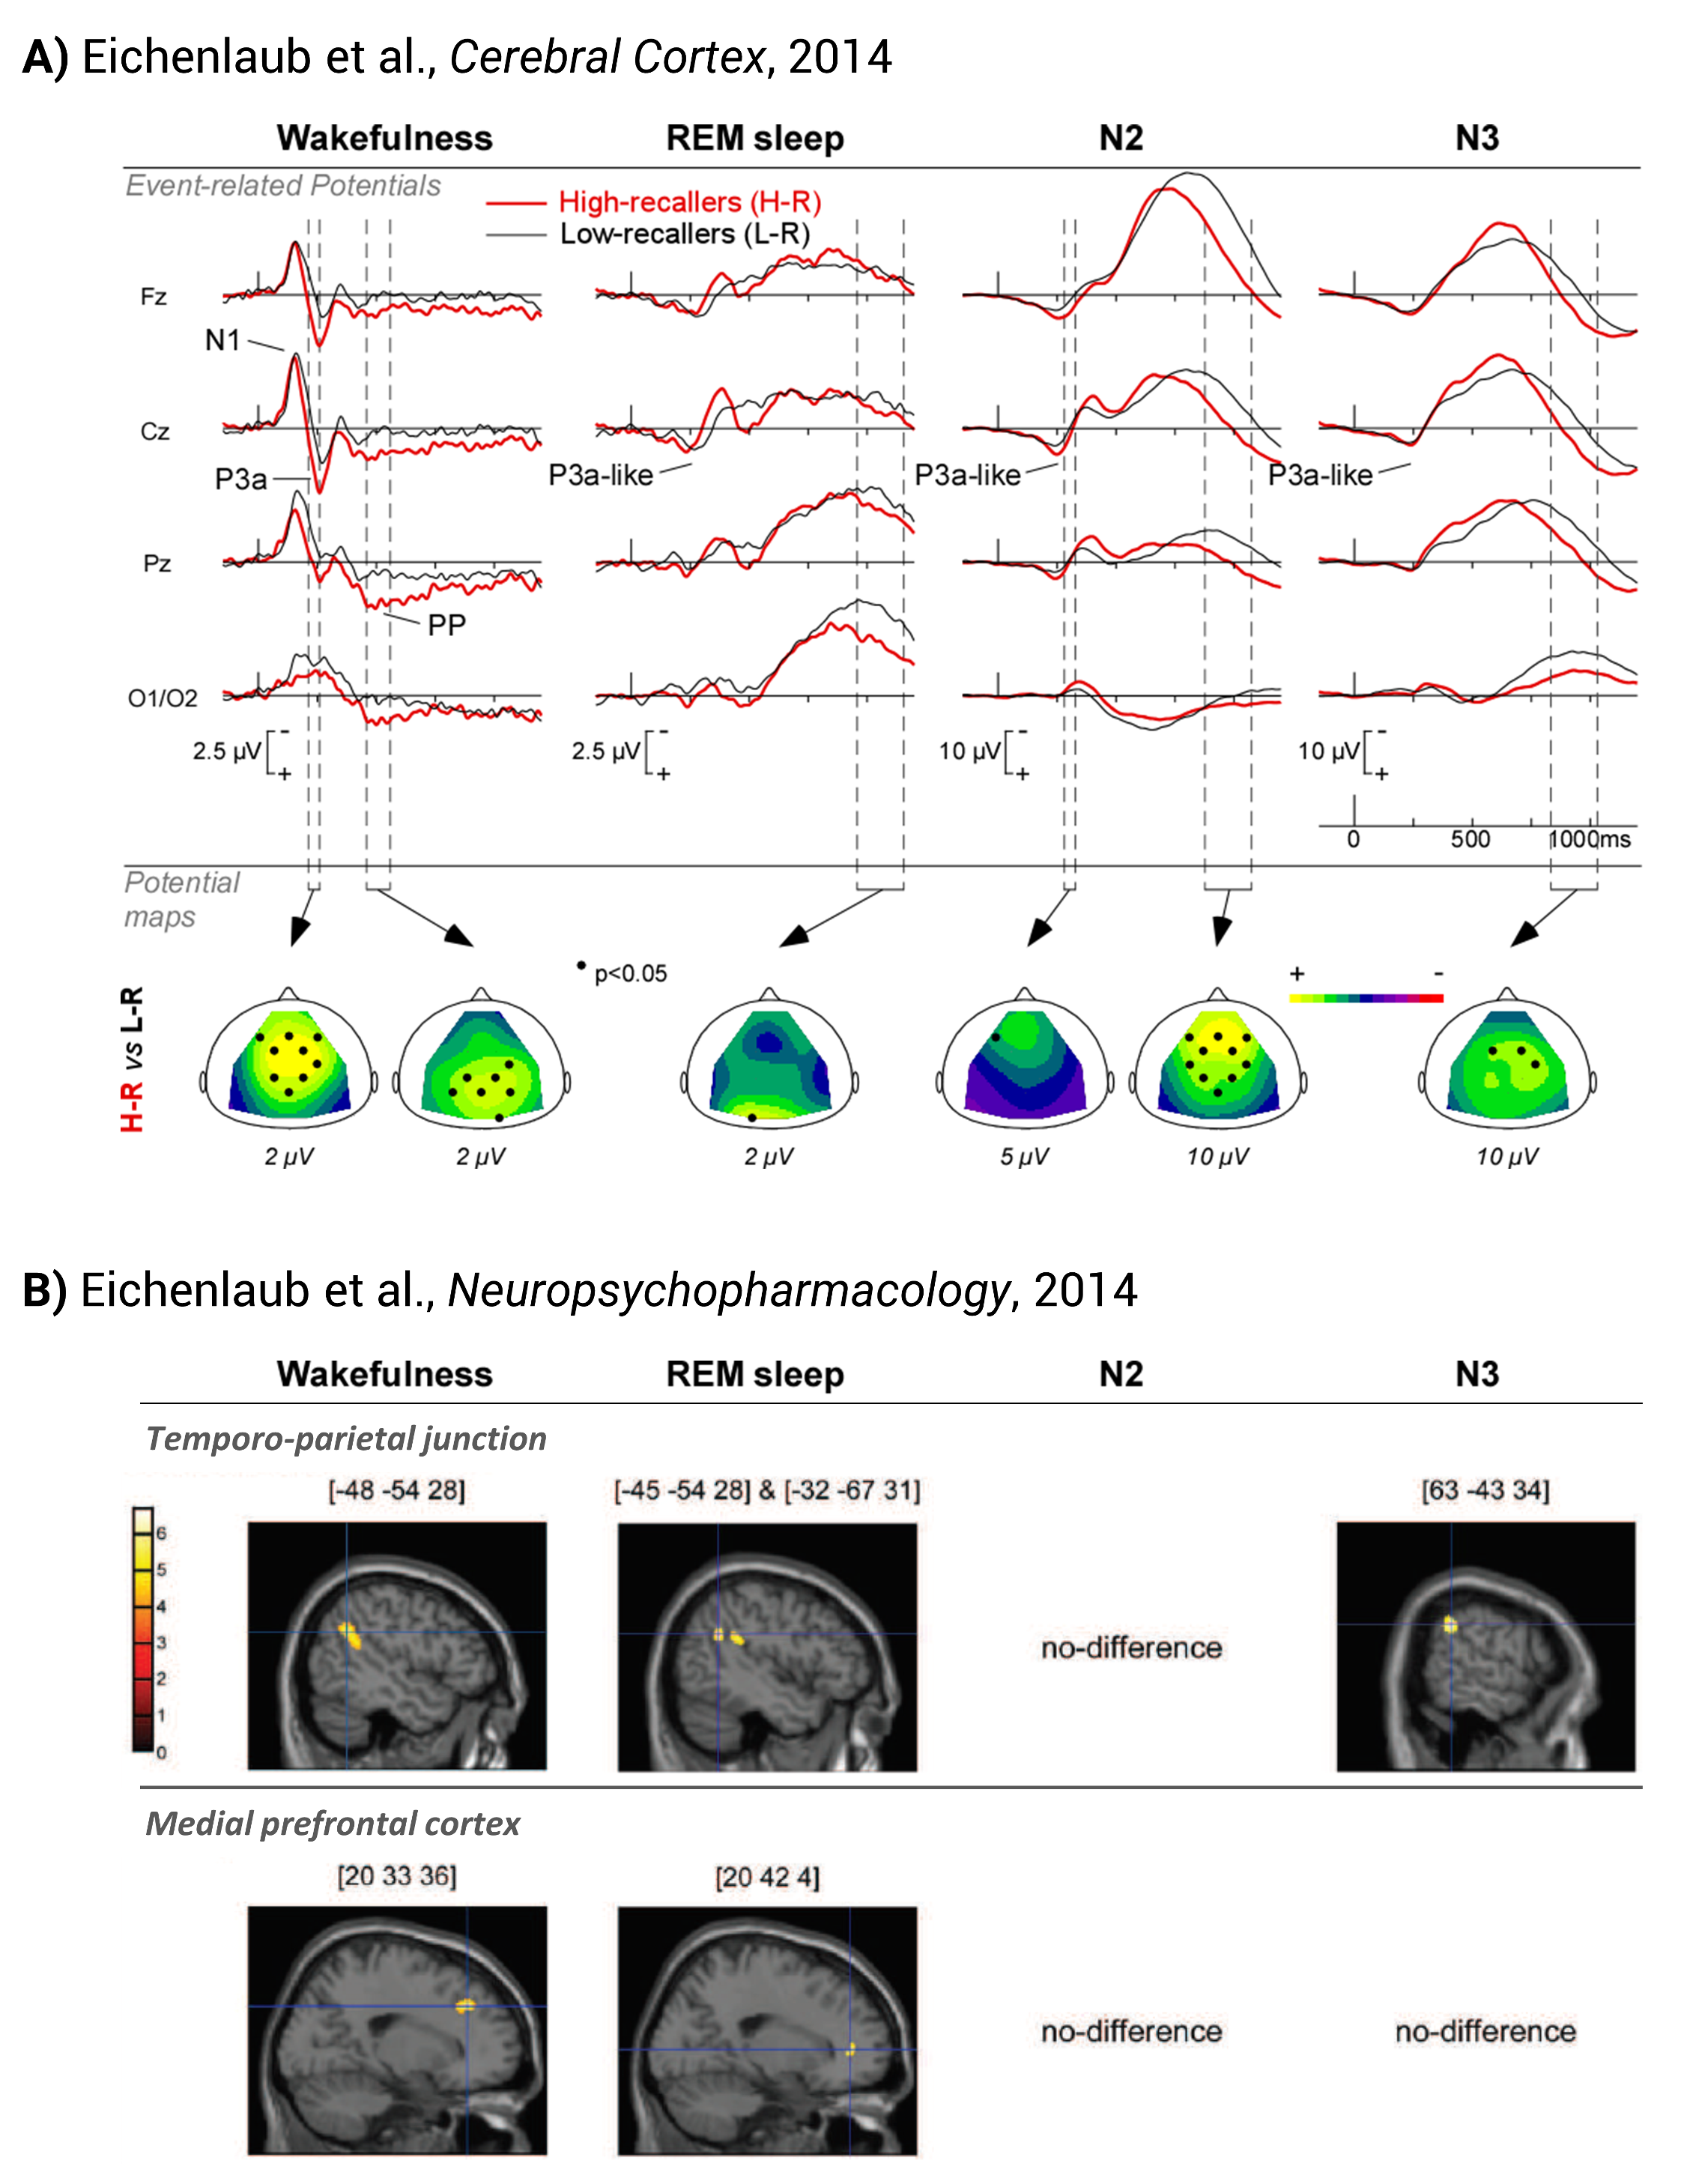
\includegraphics[width=\textwidth]{Fig/Intro/Intro_JBE_summary/Intro_JBE_summary.png}
	\caption[Summary of the results obtained in Eichenlaub's PhD thesis]{Summary of the results obtained in Eichenlaub's PhD thesis}
	\label{fig:intro:jbe-summary}
\end{figure}

\subsection{Link between neurophysiological and psychological traits}
\label{sec:dream-recall:param:link}

In conclusion, we have seen that many parameters covary with DRF. The ability to recall dreams seems to be associated with psychological and personality factors on one hand, and neurophysiological trait factors on the other hand. These results should be regarded as complementary rather than contradictory. For instance, the fact that HRs demonstrate higher rCBF during sleep and wakefulness in the TPJ and MPFC, two regions of the DMN, is consistent with the DMN hypothesis of dreaming, and is well in line with the finding that HRs are more often absorbed in their inner worlds (i.e. day-dreaming, fantasy) and more anxious. Indeed, studies have reported a positive correlation between the activity of the MPFC during wakefulness and scores of openness to experience \citep{sutin_sex_2009} and neuroticism \citep{zald_brain_2002}.

\section{Theories on dream recall}
\label{sec:dream-recall:theories}

This section summarizes the main theories to explain variability in DRF (see also \citealp{schredl_dream_1996}).

\subsection{Freud’s repression hypothesis}
\label{sec:dream-recall:theories:freud}

Freud believed that the function of dreams is to preserve sleep by representing as fulfilled wishes that would otherwise awaken the dreamer. According to him, \q{the forgetting of the dream is in a large measure the work of the resistance} \citep{freud_interpretation_1900}, which means that dreams that are not sufficiently disguised to pass the censor will be entirely repressed and therefore forgotten. However, as highlighted by \citet{schredl_dream_1999}, it is impossible to test this hypothesis because we cannot measure the non-recalled dreams in order to compare them to the recalled ones.

\subsection{Life-style hypothesis}
\label{sec:dream-recall:theories:life-style}

Schonbar was one of the first to investigate the psychological correlates of differential DRF. She proposed that DRF can be better explained as part of a general life-style and personality traits \citep{schonbar_differential_1965}. According to her work, high dream recallers are characterized by an ‘inner-acceptant’ life-style, which involves higher creativity, introspection, fantasy proneness and openness to experience. This hypothesis has been corroborated by several experimental studies that reported a positive association between DRF on one hand and openness to experience, absorption and creativity on the other hand (see section \ref{sec:dream-recall:param:link}).

\subsection{Salience hypothesis}
\label{sec:dream-recall:theories:salience}

Based on the idea that the principles of waking memory apply to dream recall, Cohen developed in the seventies the interference hypothesis \citep{cohen_dream_1973} followed by the salience hypothesis \citep{cohen_test_1974}. The interference hypothesis postulates that the dream memory trace remains so long as there is no distraction or interference. Otherwise, dreams are forgotten in order to maximize the memory capacity for the day ahead. This echoes French philosopher Roger Caillois’s idea on dream forgetting: \q{Dreams are quickly forgotten because they have no consequences on waking life and there is only benefits in forgetting them} \citep{caillois_incertitude_1956}. In more practical terms, the central idea of this theory is that the dreamer must voluntary pay attention to the dream immediately after awakening. In this respect, it overlaps the life-style hypothesis since high dream recallers are expected to be more interested in their dreams and therefore put more attention on them upon awakening.
Cohen further extended his model in the salience hypothesis, which emphasizes dream content and states that the more salient a dream (e.g. a vivid, bizarre, and highly emotional dream), and the less interferences there are during the recall process, the more likely the dream is to be recalled. Several findings are in favor of this hypothesis. For example, it has been shown that bizarreness \citep{cipolli_bizarreness_1993} and emotionality \citep{schredl_emotions_1998} enhance recall of dream content (an observation that was however not replicated when taking the effect of dream length into account; \citealp{schredl_relationship_2000}). More recently, \citet{parke_re-examination_2009} have studied the combined effect of interference and salience processes on dream recall. The findings suggest that a link is present, as the more interference experienced has tended to reduce the length of the dream recall in turn reducing the reported salience.

\subsection{Arousal-retrieval model}
\label{sec:dream-recall:theories:arousal}

\citet{koulack_dream_1976} proposed in their so-called arousal-retrieval model that a short period of wakefulness (arousal) must occur immediately after dreaming in order to transfer the dream content from short-term memory to long term memory. Furthermore, they drew on Cohen’s work to propose that the salience of dream content and lack of interferences during the recall process were critical for a successful recall of the stored dream (retrieval). The arousal-retrieval model is one of the most comprehensive model of dream recall and has received great support from the literature, reviewed earlier in section \ref{sec:dream-recall:param:sleep}.

\subsection{State-shift hypothesis}
\label{sec:dream-recall:theories:state}

Extending these arousal-based ideas, \citet{koukkou_dreaming:_1983} proposed the state-shift hypothesis which emphasizes the state dependent effects of dream recall rather than short-term memory effects. According to them, \q{forgetting of dreams is a function of the magnitude of the difference between states during encoding and recall} \citep{koukkou_dreaming:_1983}. Consequently, the closer two functional states are, the better is the transference of information. Thus, dreams are only recalled when the awake functional state
is similar to the sleeping functional state. It was argued that such compatibility occurs between wakefulness and REM sleep, enabling better recall of REM dreams. By contrast, the slow EEG frequencies of NREM sleep (and especially N3 sleep) are functionally very different from wakefulness, and this could account for the poorer NREM dream recall.

\subsection{Sleep inertia}
\label{sec:dream-recall:theories:inertia}

\citet{conduit_poor_2004} demonstrated that the performance during or shortly after awakening is of importance for the process of dream recall. The design of their study is as follows. Participants were instructed to produce an eye movement signal whenever they heard a tone, presented at increasing volume during N2 and REM sleep until an eye movement signal verification was observed.  Ninety seconds after signal verification, participants were awakened and asked if they remembered hearing the tone or responding with the EM signal. Such recollection of signal verified tone presentations was significantly less after Stage 2 sleep (65\%) compared to REM sleep (100\%) presentations. Furthermore, signal verified tone recall was significantly correlated with reported dream recall frequency. They concluded that \q{quite possibly, brain functioning underlying the reporting and non-reporting of dreams does not exist within the pre-sleeping period at all, but within the period just after awakening, when cognitive resources are in demand to recall and/or consolidate events which have just occurred within the previous sleeping period} \citep{conduit_poor_2004}.
Echoing these findings, \citet{schredl_factors_2003} noted that cognitive functioning in the period just after awakening is often severely impaired (an effect referred to as sleep inertia; \citealp{tassi_sleep_2000, trotti_waking_2016}), and that it would be in consequence \q{promising to correlate inter-individual differences regarding the sleep inertia with DRF}. This issue will form a large part of the doctoral work hereby presented and we will return to this in section \ref{sec:problematic:inertia}.

\subsection{Towards a unifying theory of dream recall}
\label{sec:dream-recall:theories:unifying}

This brief overview leads to the observation that there is a broad spectrum of dream recall theories, ranging from relating to the content of the dream (Freud’s repression and Cohen’s salience hypotheses) to accounting for the psychological (life-style hypothesis), cognitive and physiological processes (arousal-retrieval,  state-shift hypothesis, sleep inertia; see Figure \ref{fig:intro:dream-recall-models}). The empirical data seems hitherto to fit best into the arousal-retrieval model (which integrates elements of both the Salience and Interference hypotheses) and the life-style hypothesis. A comprehensive, unified theory of dream recall should combine these two models, for example using the arousal-retrieval model to account for day-to-day variability in DRF (state factors), and the life-style hypothesis to account for the large inter-individual DRF variability (traits factors). Moreover, there is a currently a lack of evidence for the state-shift hypothesis (due to the difficulty of deriving valid quantitative measures for the closeness of functional states; \citealp{schredl_dream_1999}) and the sleep inertia theory, which both insist on brain functioning within the period just after awakening.

\begin{figure}[htb]
	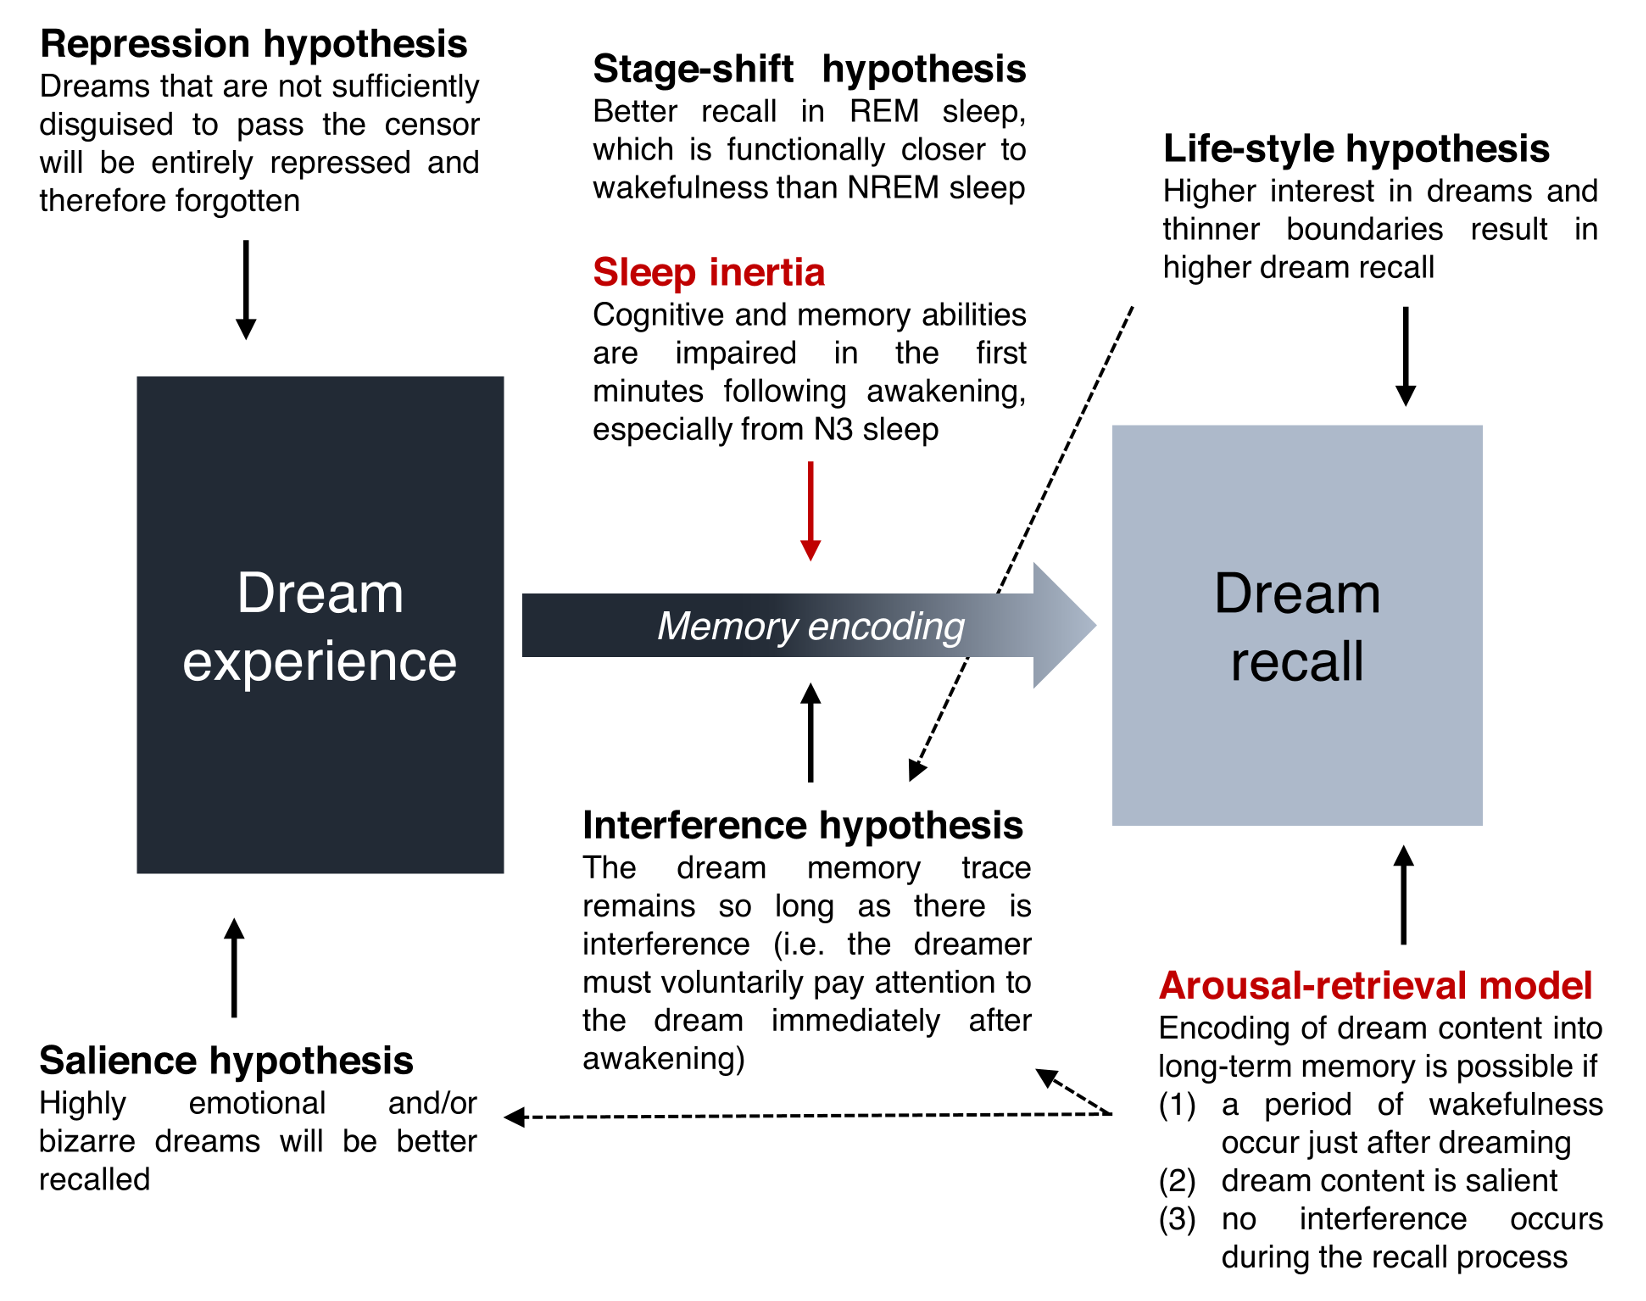
\includegraphics[width=\textwidth]{Fig/Intro/Intro_DRF_model/Intro_DRF_model.png}
	\caption[Dream recall theories]{Dream recall theories. The arousal-retrieval model provides so far the most comprehensive theory on dream recall and is firmly grounded in empirical evidence. At its simplest, it states that a short period of wakefulness must occur just after dreaming (arousal) in order to transfer the dream content from short to long term memory, which is otherwise impossible during sleep. In addition, it postulates that the dream content must be salient (Salience hypothesis, e.g. highly emotional, vivid and/or bizarre) and that the dreamer must voluntarily pay attention to the dream content (Interference hypothesis). Notably, it is very probable that the individuals with the greatest interest in dreams (Life-style hypothesis) are also the ones which focus the more on their dreams immediately after awakening, thus reducing encoding interferences. This would provide a link between the Life-style hypothesis and the arousal-retrieval model. Finally, sleep inertia could be a important explanatory factor with regards to DRF. It is possible that low dream recallers experience more acute sleep inertia upon awakening, whatever the sleep stage before awakening. More impaired memory and cognitive abilities upon awakening would in turn prevent the encoding of dreams to long term-memory. However, this hypothesis remains to be tested empirically.}
	\label{fig:intro:dream-recall-models}
\end{figure}
